\section{Mô hình Use Case và Đặc tả Use Case}
Phần này trình bày hệ thống sơ đồ Use Case tổng quát và chi tiết theo từng phân hệ chức năng của LumiCinema, kèm theo bảng đặc tả chi tiết từng Use Case đồng bộ với mã nguồn thực tế.

\subsection{Hệ thống sơ đồ Use Case}
\begin{figure}[H]
  \centering
  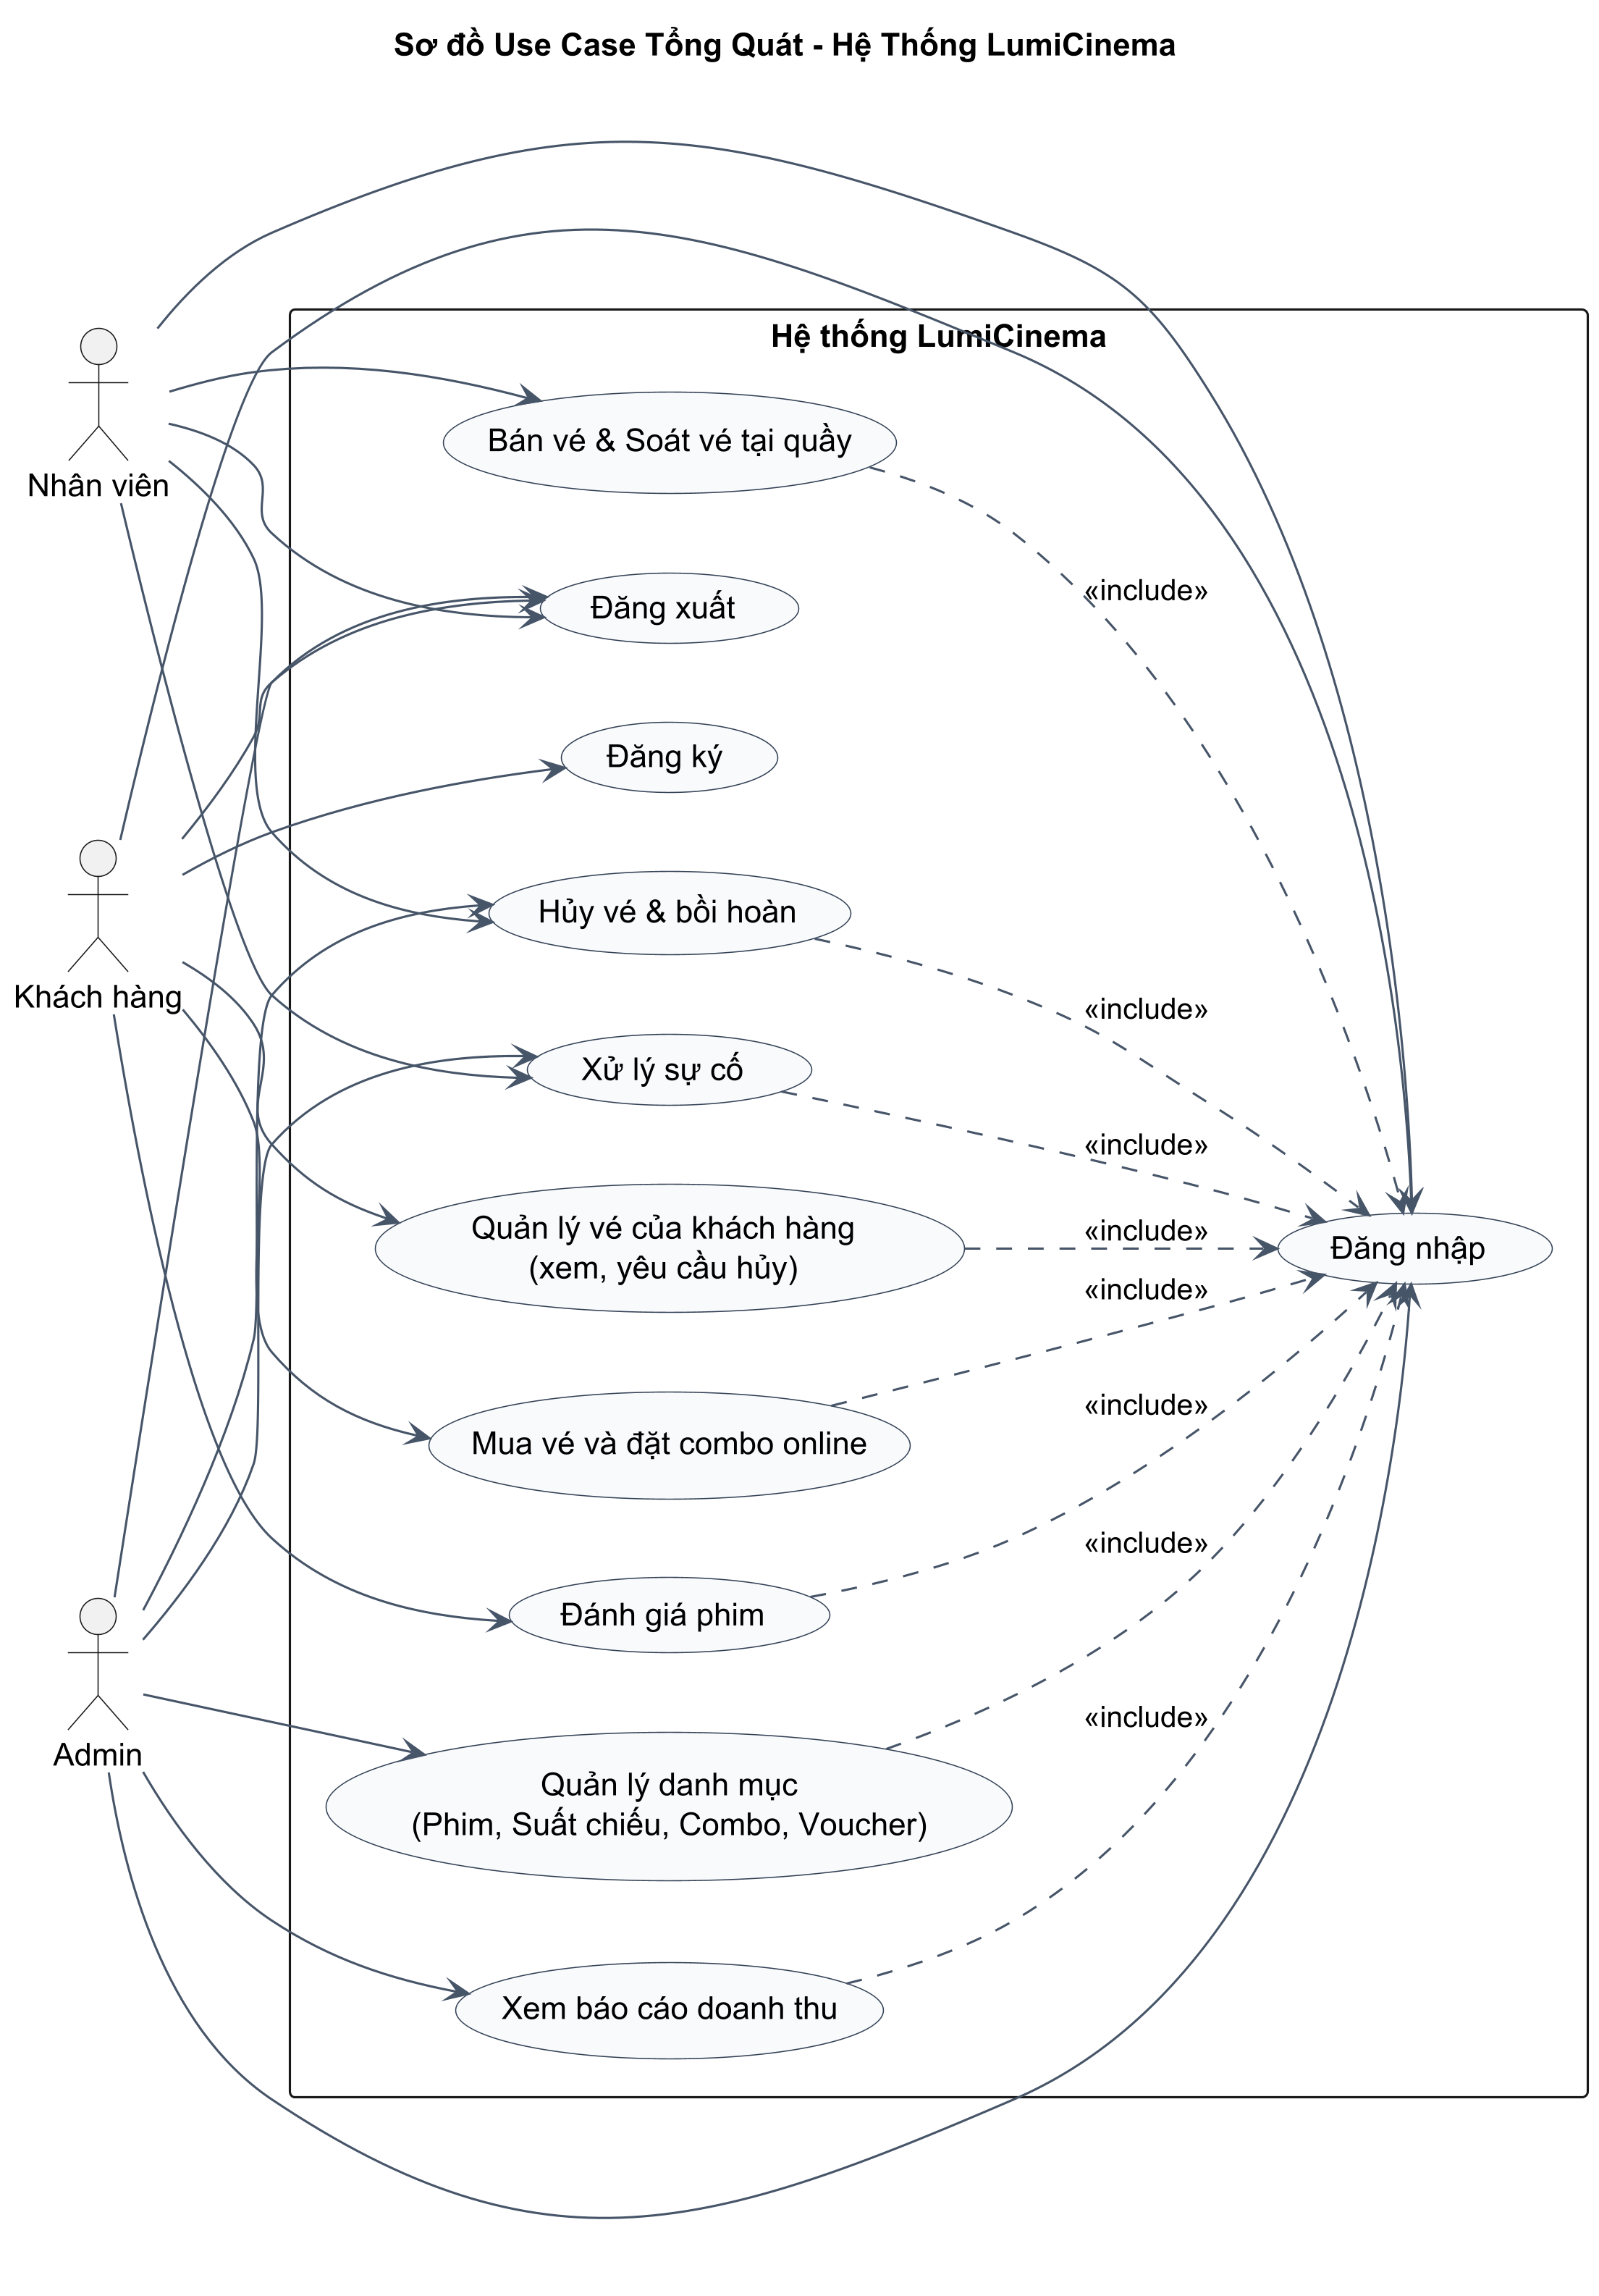
\includegraphics[width=\textwidth,height=0.80\textheight,keepaspectratio]{images/usecase/2.2_usecase_tong_quat.png}
  \caption{Sơ đồ Use Case Tổng Quát - Hệ Thống LumiCinema}
  \label{fig:uc_01}
\end{figure}

\begin{figure}[H]
  \centering
  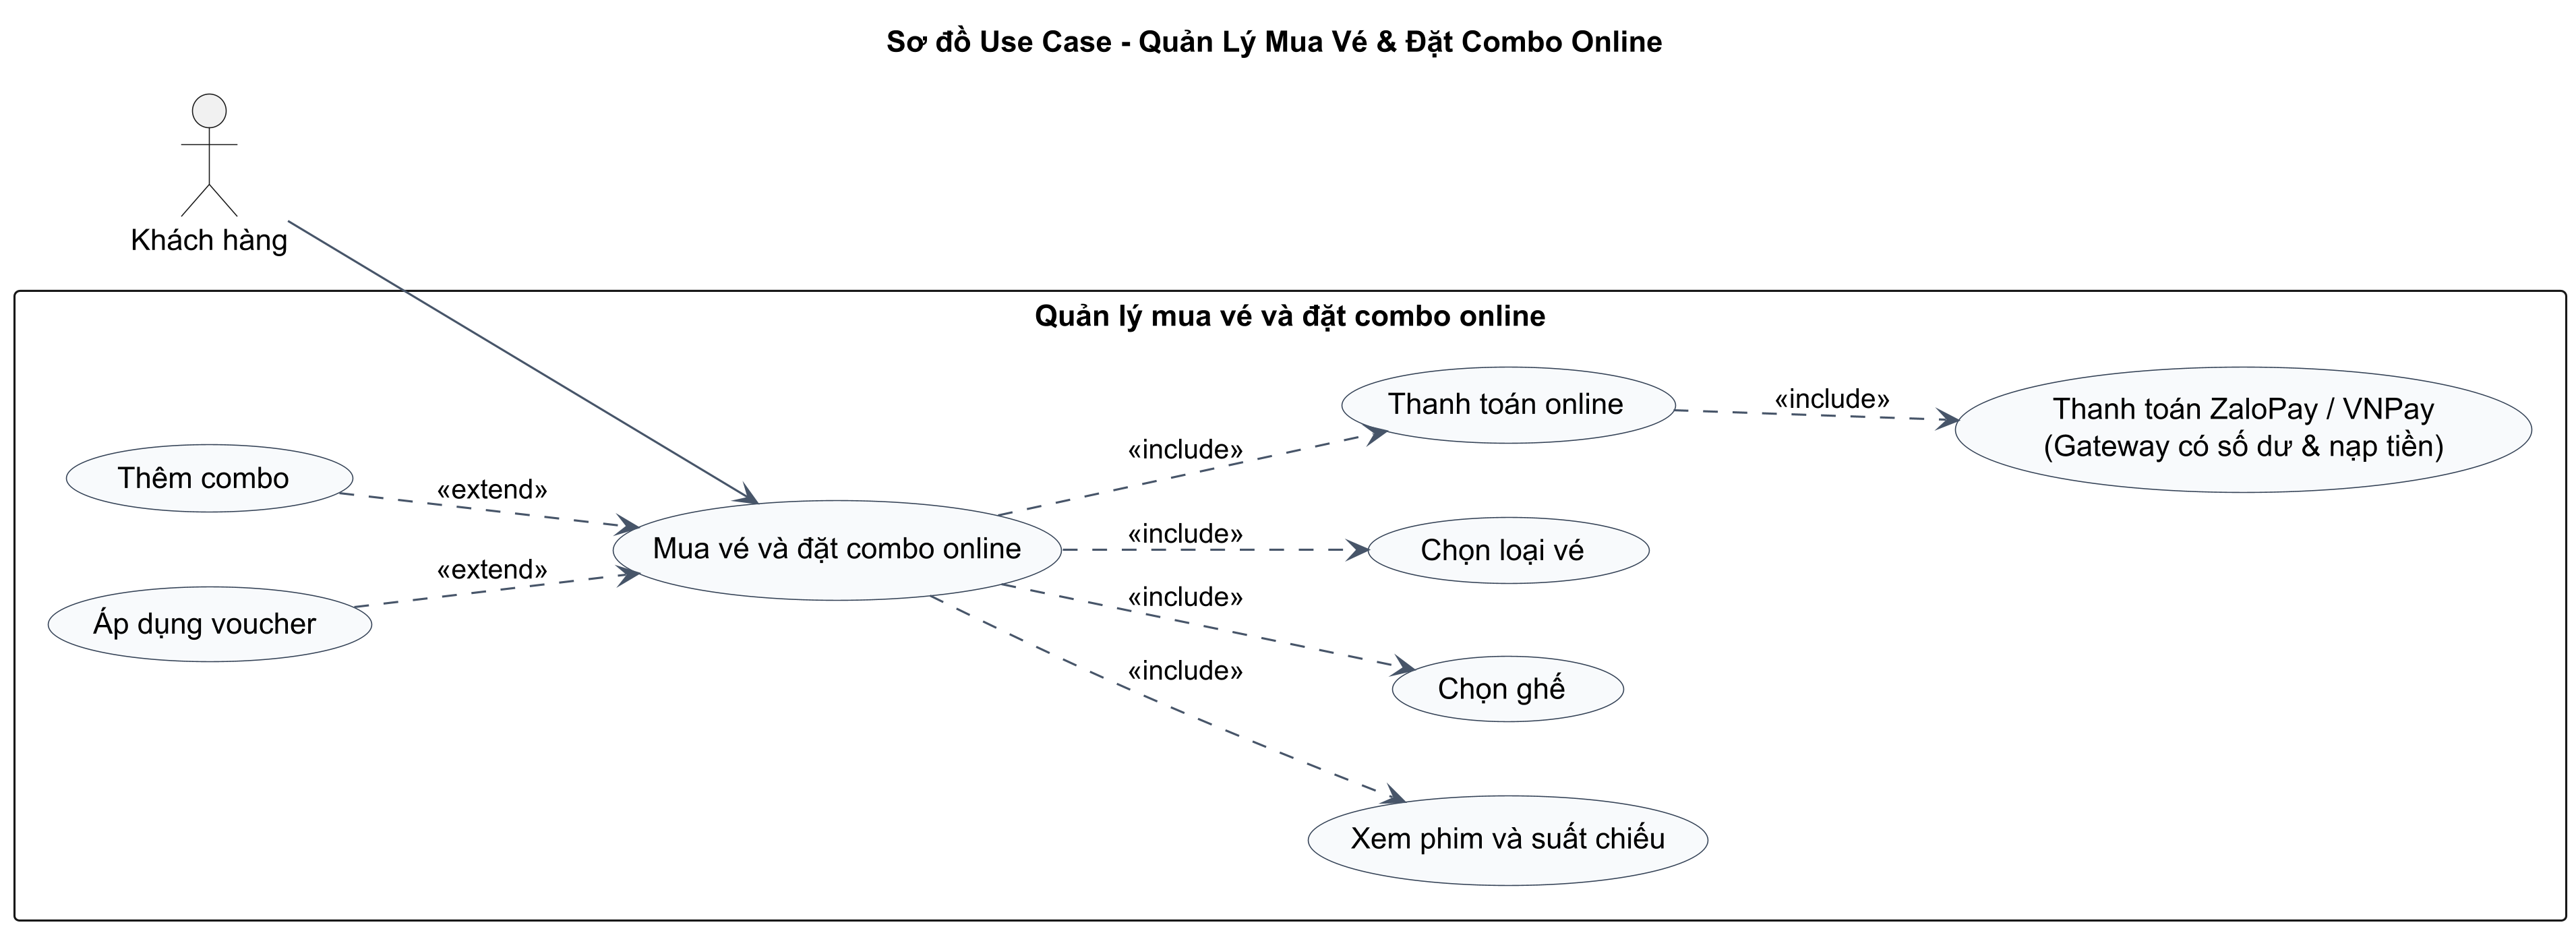
\includegraphics[width=\textwidth,height=0.80\textheight,keepaspectratio]{images/usecase/2.3_usecase_mua_ve_dat_combo_online.png}
  \caption{Sơ đồ Use Case - Quản Lý Mua Vé \& Đặt Combo Online}
  \label{fig:uc_02}
\end{figure}

\begin{figure}[H]
  \centering
  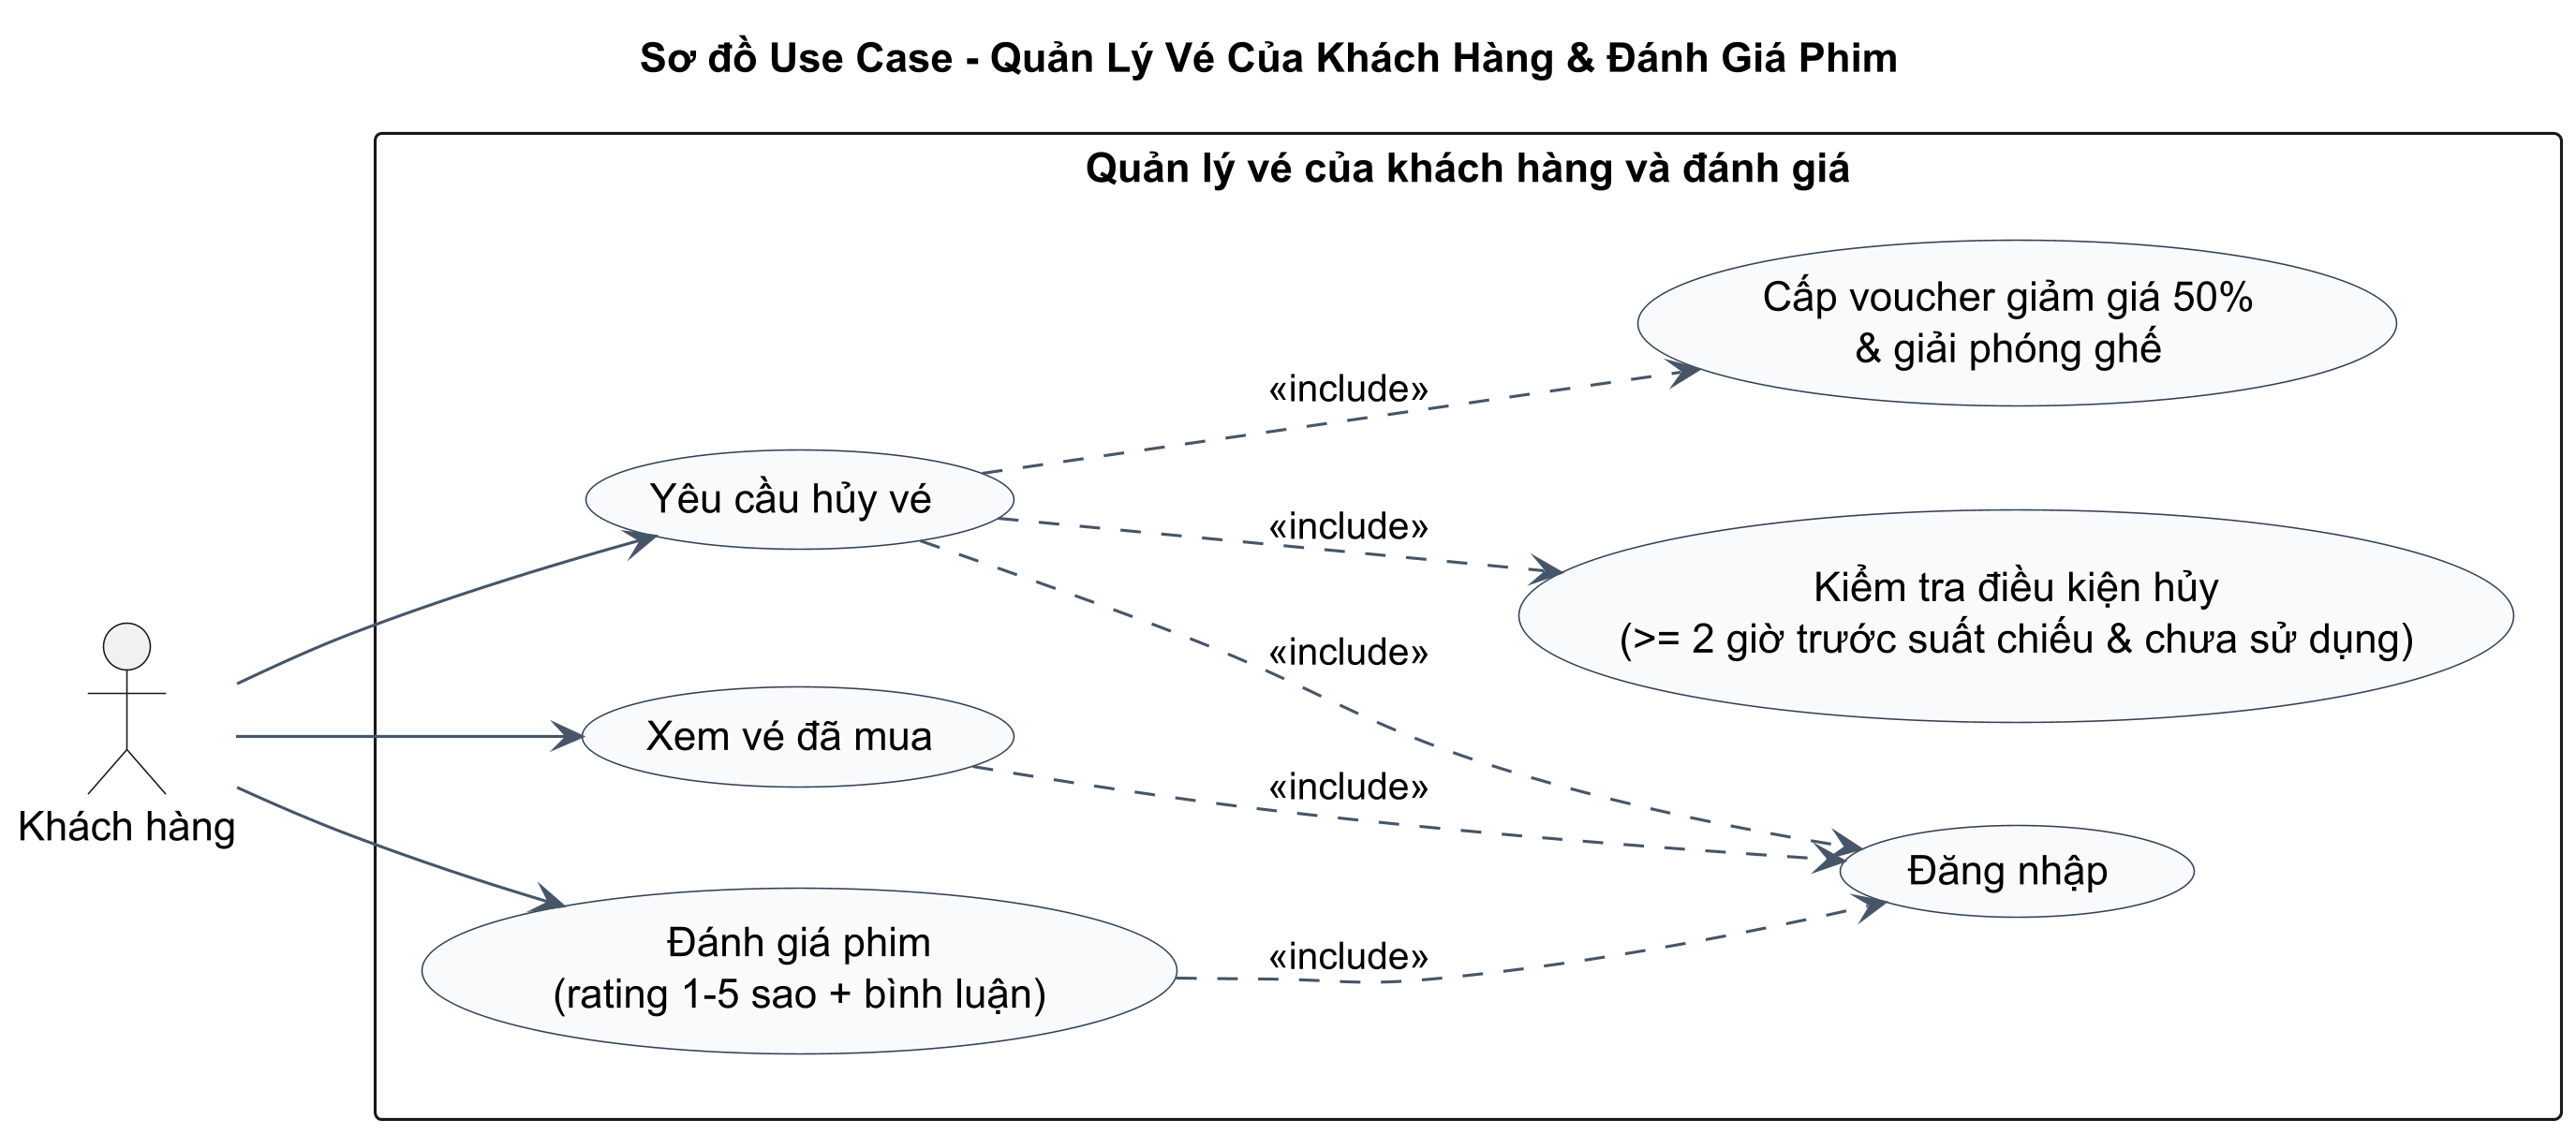
\includegraphics[width=\textwidth,height=0.80\textheight,keepaspectratio]{images/usecase/2.4_usecase_quan_ly_ve_va_danh_gia.png}
  \caption{Sơ đồ Use Case - Quản Lý Vé Của Khách Hàng \& Đánh Giá Phim}
  \label{fig:uc_03}
\end{figure}

\begin{figure}[H]
  \centering
  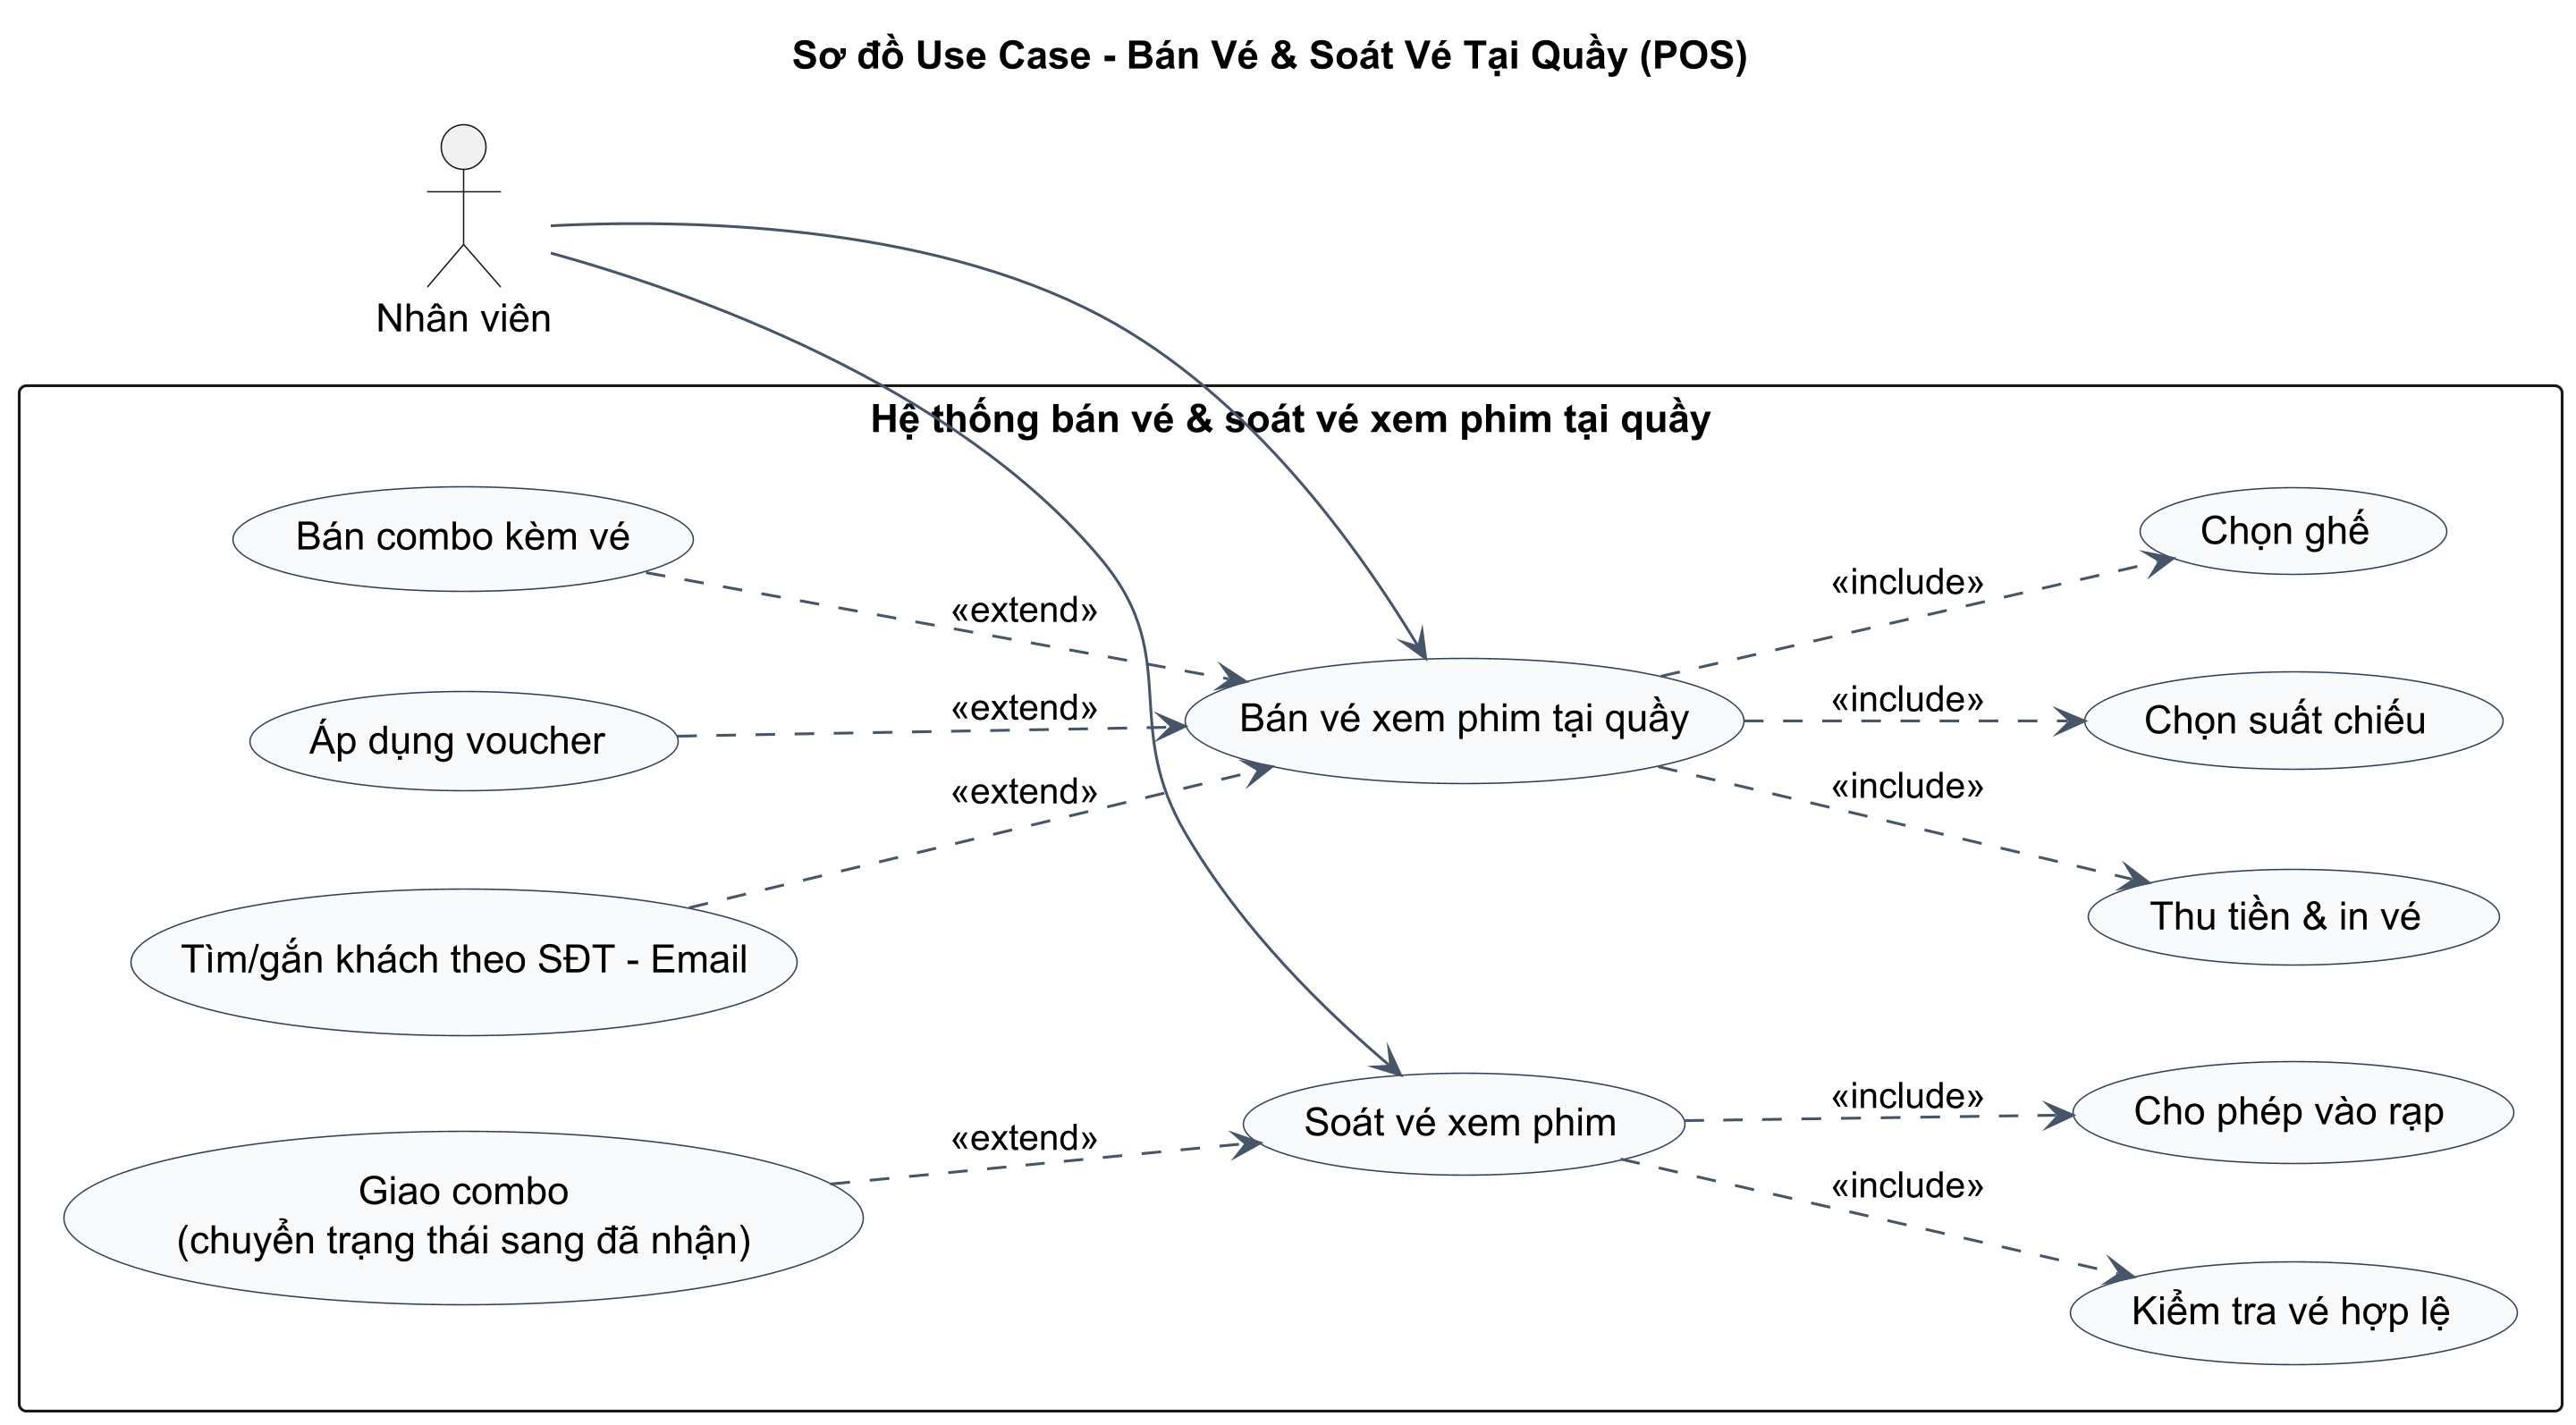
\includegraphics[width=\textwidth,height=0.80\textheight,keepaspectratio]{images/usecase/2.5_usecase_ban_ve_soat_ve_tai_quay.png}
  \caption{Sơ đồ Use Case - Bán Vé \& Soát Vé Tại Quầy (POS)}
  \label{fig:uc_04}
\end{figure}

\begin{figure}[H]
  \centering
  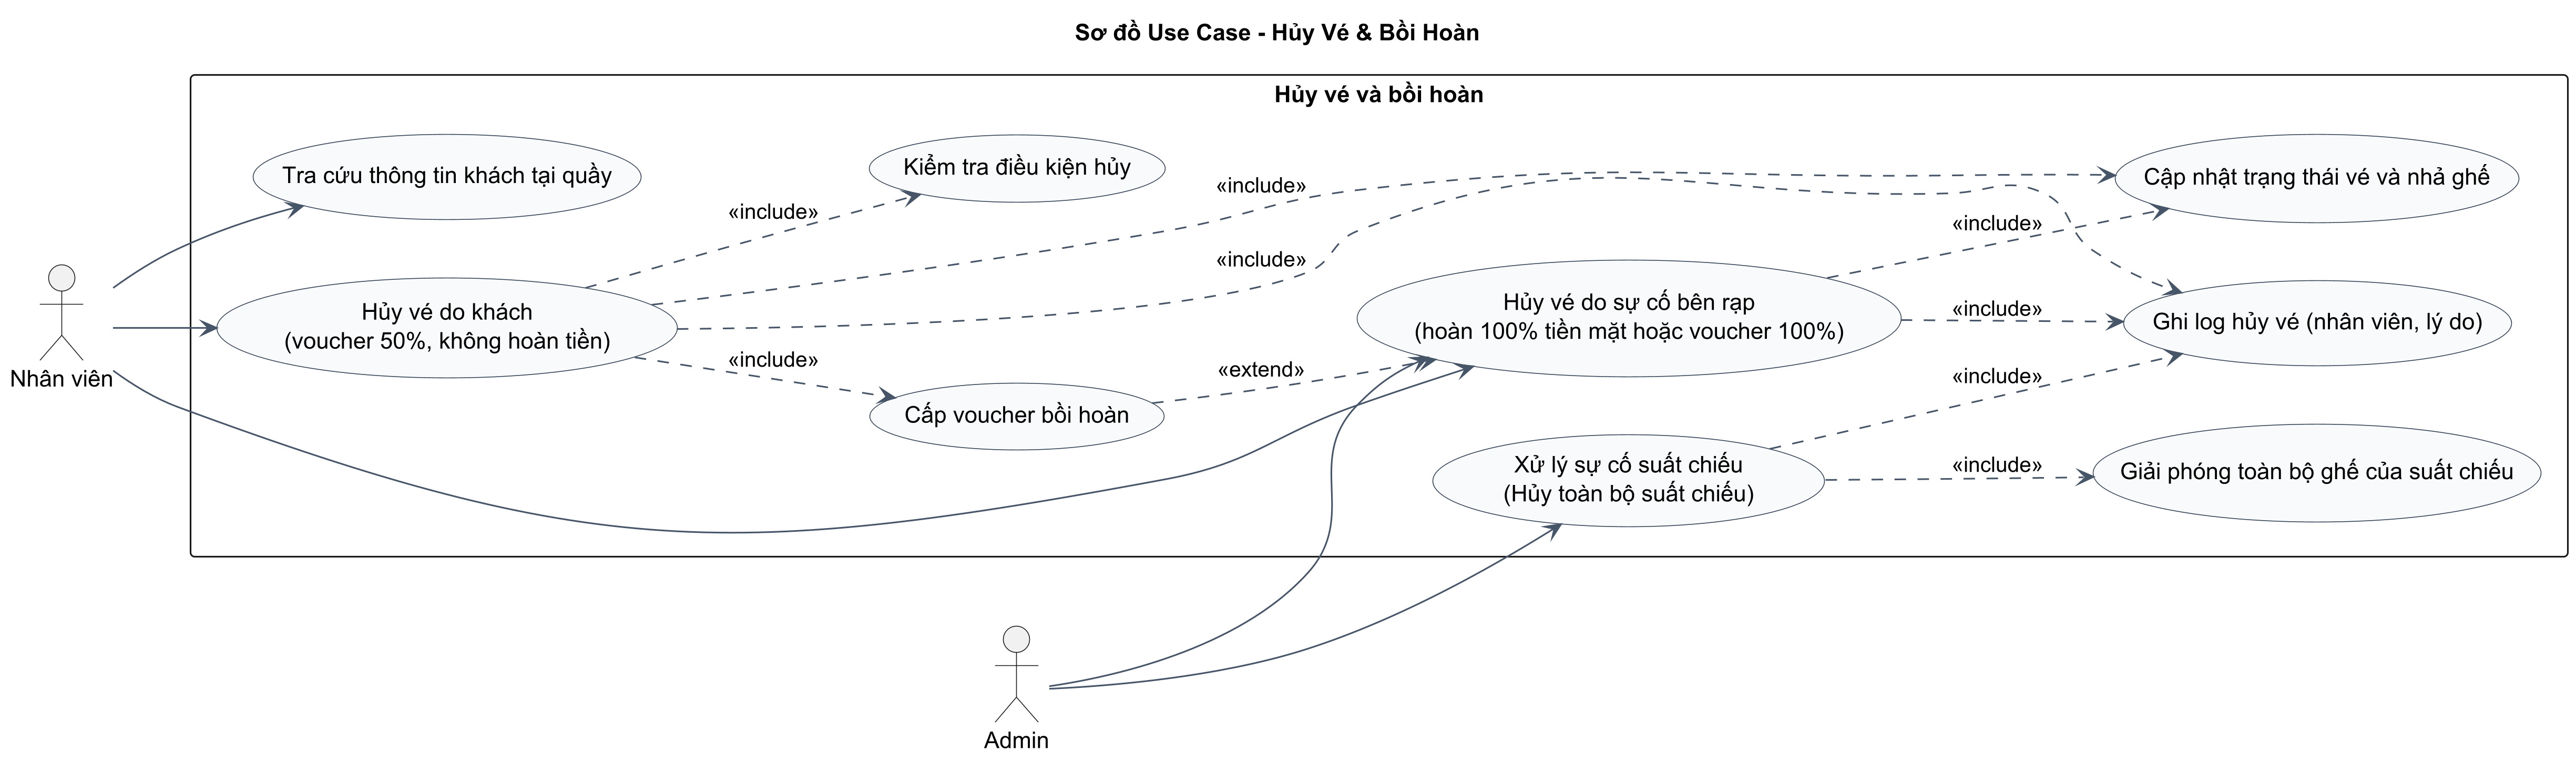
\includegraphics[width=\textwidth,height=0.80\textheight,keepaspectratio]{images/usecase/2.6_usecase_huy_ve_va_boi_hoan.png}
  \caption{Sơ đồ Use Case - Hủy Vé \& Bồi Hoàn}
  \label{fig:uc_05}
\end{figure}

\begin{figure}[H]
  \centering
  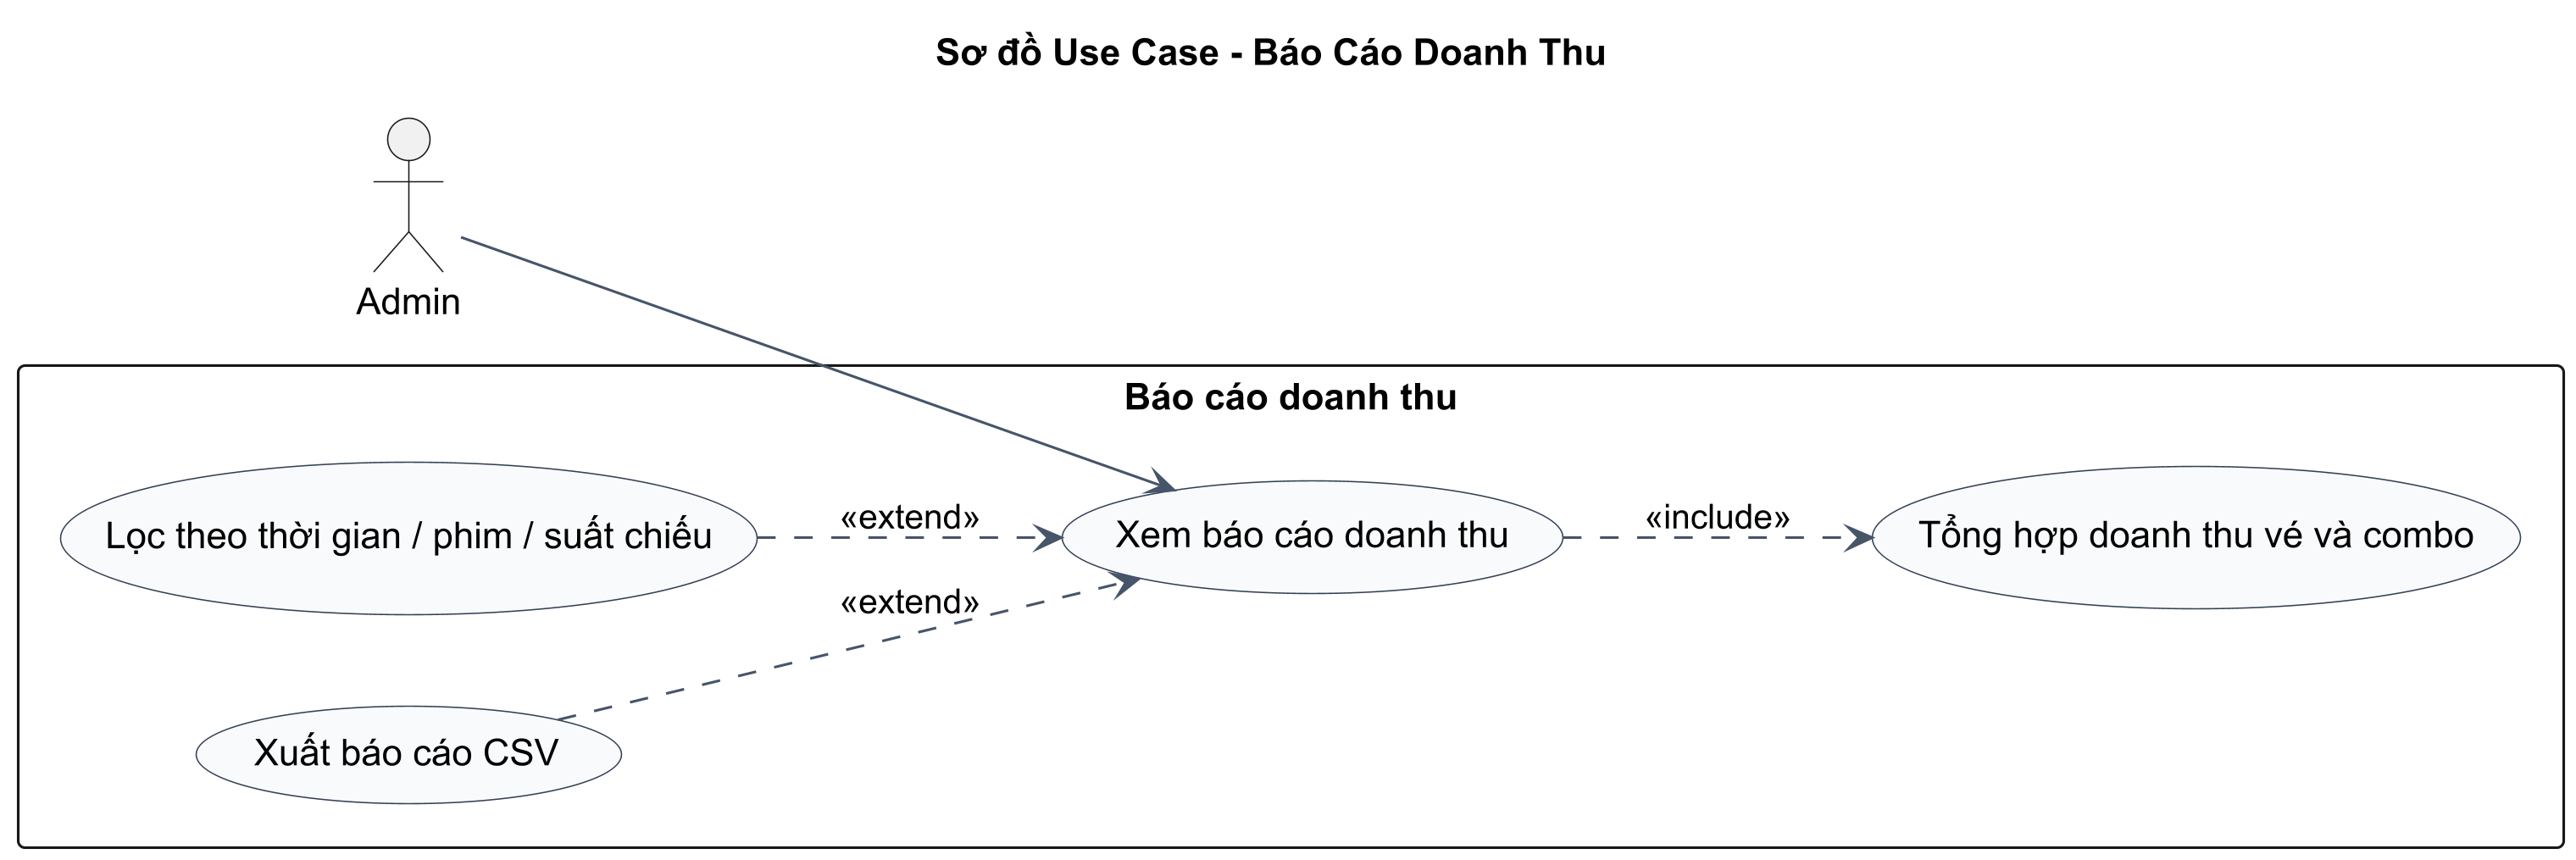
\includegraphics[width=\textwidth,height=0.80\textheight,keepaspectratio]{images/usecase/2.7_usecase_bao_cao_doanh_thu.png}
  \caption{Sơ đồ Use Case - Báo Cáo Doanh Thu}
  \label{fig:uc_06}
\end{figure}

\begin{figure}[H]
  \centering
  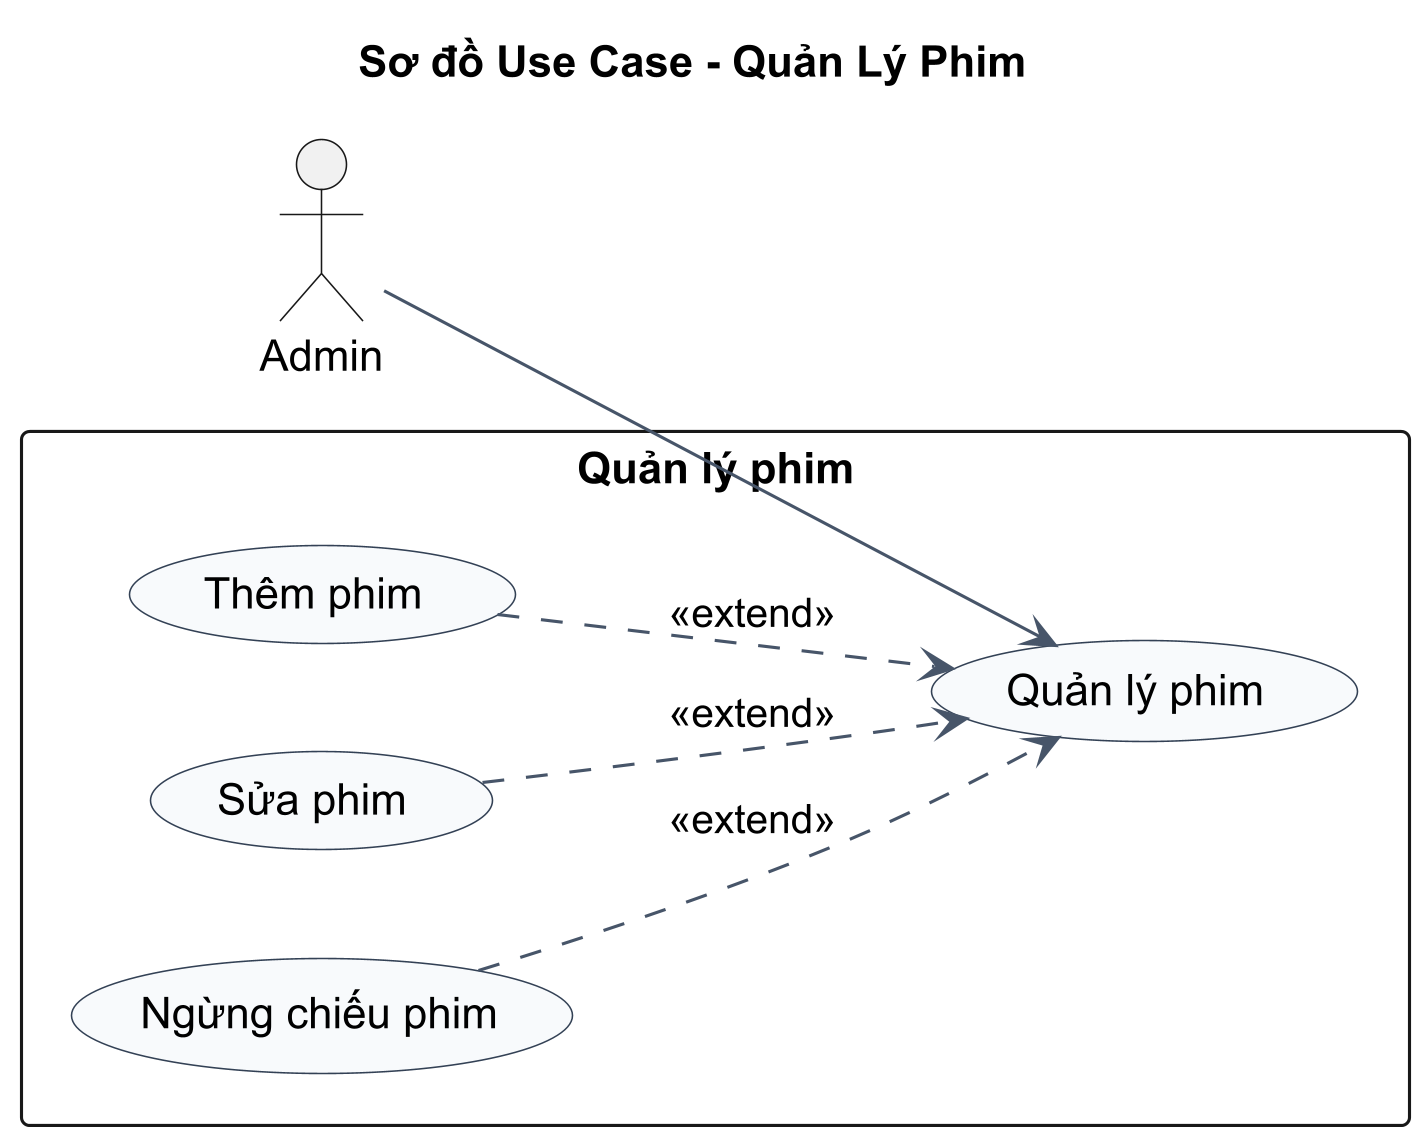
\includegraphics[width=\textwidth,height=0.80\textheight,keepaspectratio]{images/usecase/2.8_usecase_quan_ly_phim.png}
  \caption{Sơ đồ Use Case - Quản Lý Phim}
  \label{fig:uc_07}
\end{figure}

\begin{figure}[H]
  \centering
  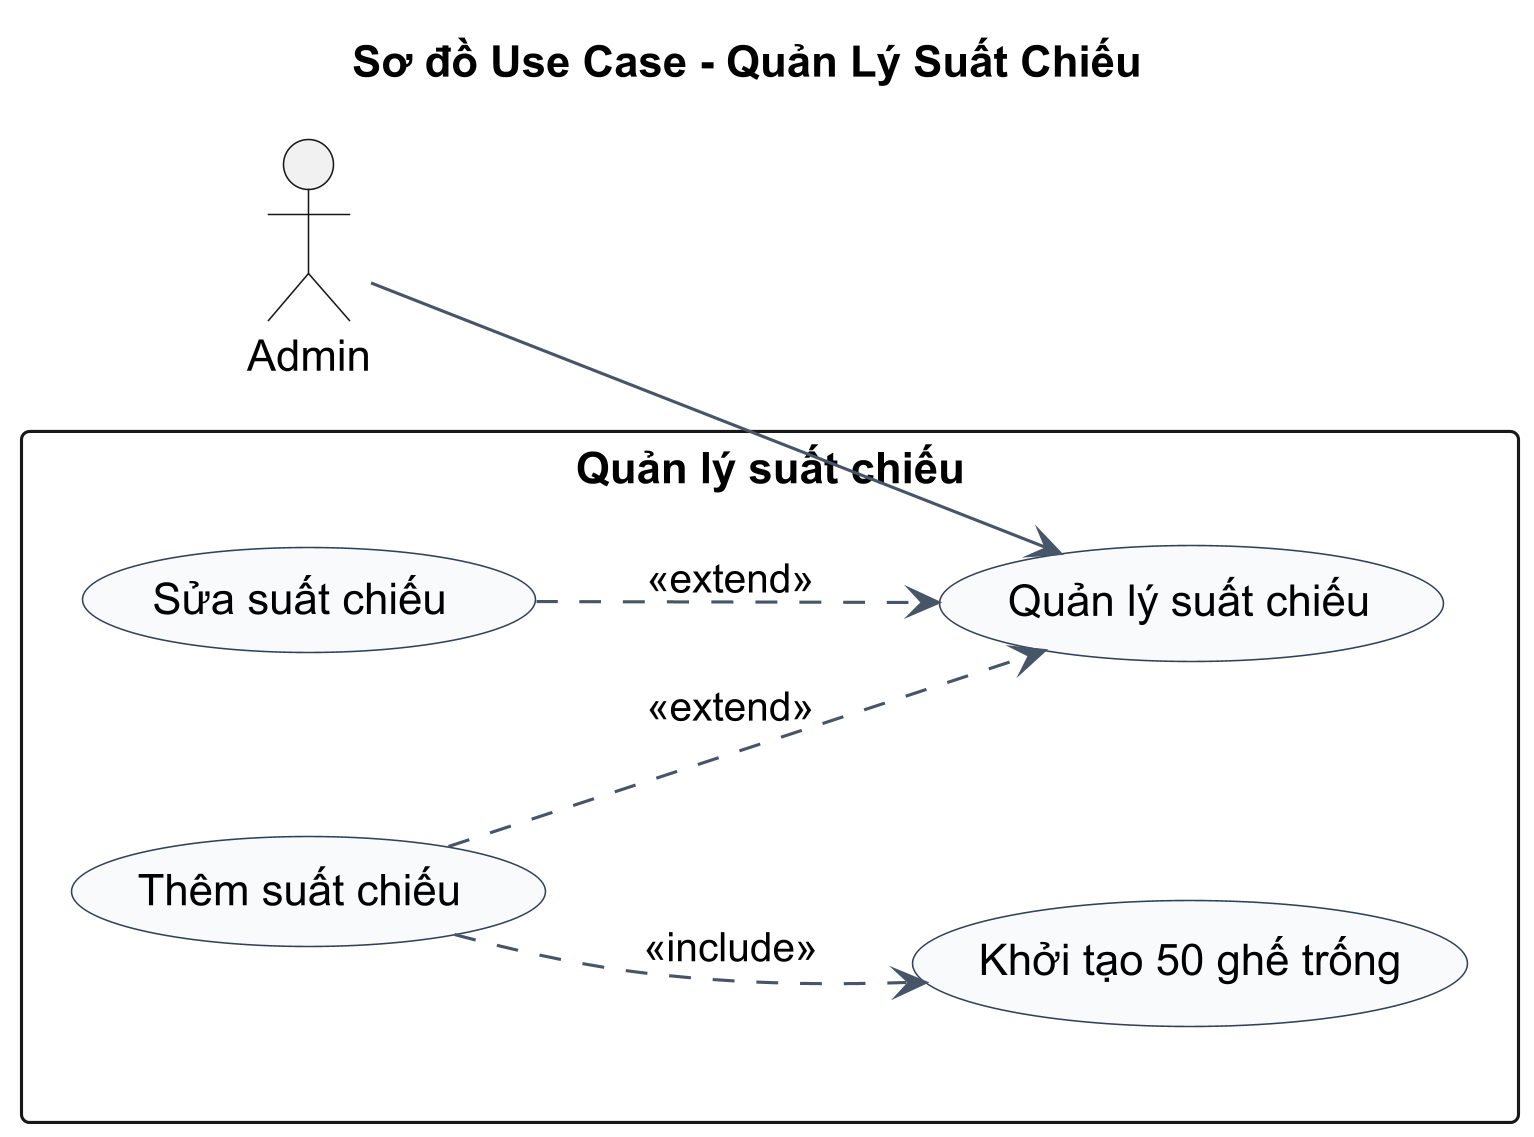
\includegraphics[width=\textwidth,height=0.80\textheight,keepaspectratio]{images/usecase/2.9_usecase_quan_ly_suat_chieu.png}
  \caption{Sơ đồ Use Case - Quản Lý Suất Chiếu}
  \label{fig:uc_08}
\end{figure}

\begin{figure}[H]
  \centering
  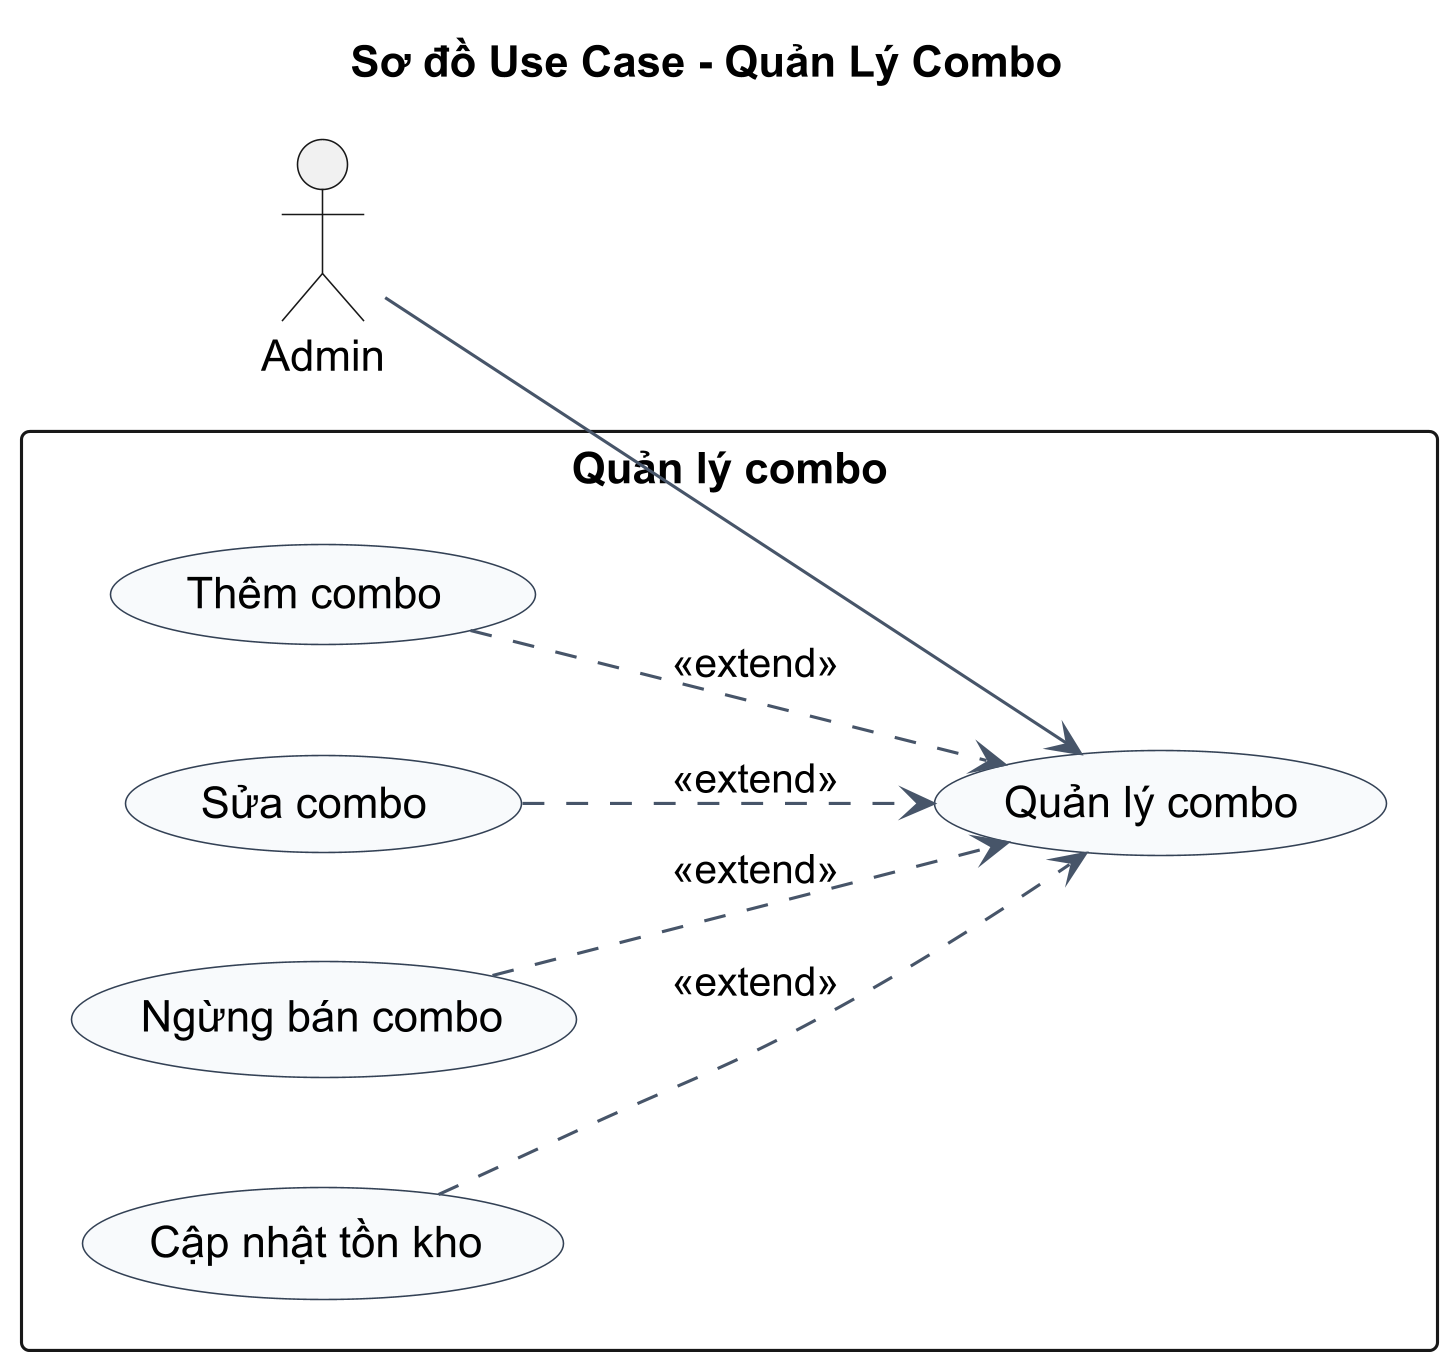
\includegraphics[width=\textwidth,height=0.80\textheight,keepaspectratio]{images/usecase/2.10_usecase_quan_ly_combo.png}
  \caption{Sơ đồ Use Case - Quản Lý Combo}
  \label{fig:uc_09}
\end{figure}

\begin{figure}[H]
  \centering
  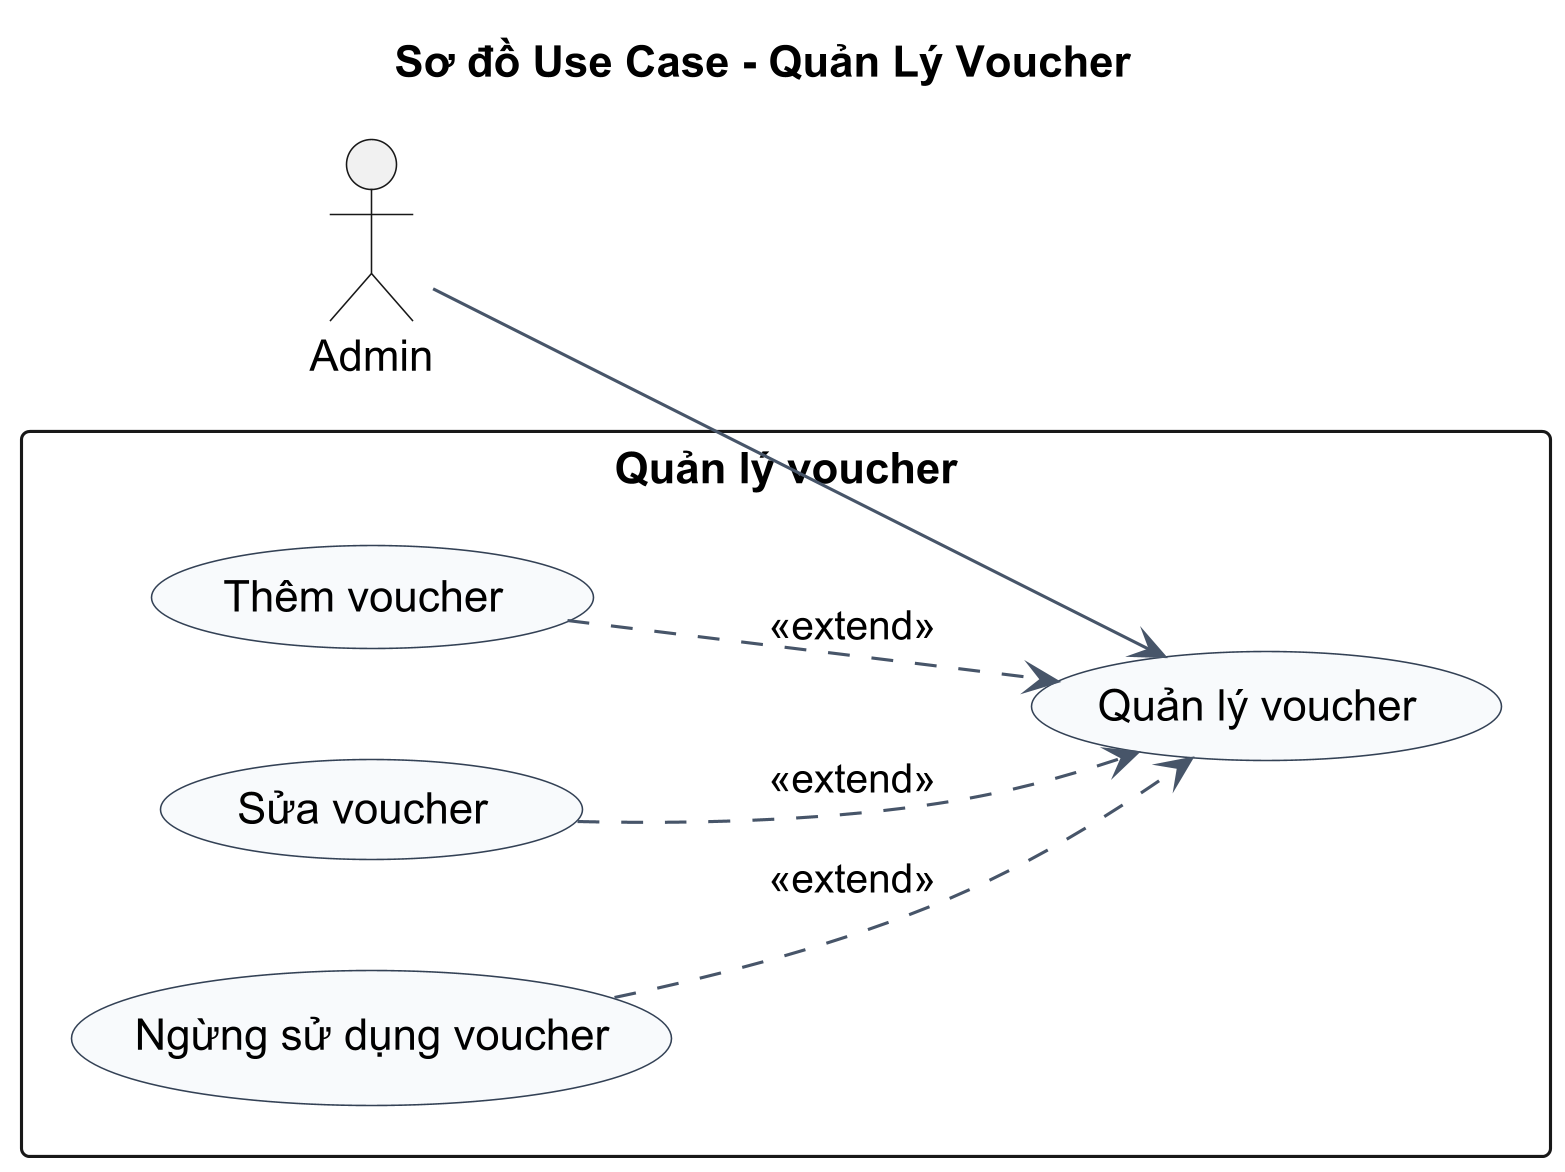
\includegraphics[width=\textwidth,height=0.80\textheight,keepaspectratio]{images/usecase/2.11_usecase_quan_ly_voucher.png}
  \caption{Sơ đồ Use Case - Quản Lý Voucher}
  \label{fig:uc_10}
\end{figure}

\subsection{Đặc tả chi tiết các Use Case}
\begin{longtable}{|p{4.2cm}|p{11.3cm}|}
\hline
\rowcolor{headerblue} \textbf{Tên Use Case} & \textbf{Quản lý vé khách hàng} \\ \hline
\endhead
\textbf{Tác nhân chính} & Admin / Người quản lý \\ \hline
\textbf{Tóm tắt} & Use Case bắt đầu khi Người quản lý truy cập chức năng quản lý vé khách hàng để xem danh sách vé, tra cứu vé, kiểm tra trạng thái và xem chi tiết vé. \\ \hline
\textbf{Dòng sự kiện chính} & 1. Người quản lý đăng nhập vào hệ thống.\newline 2. Người quản lý chọn chức năng Quản lý vé khách hàng.\newline 3. Hệ thống hiển thị giao diện quản lý vé.\newline 4. Người quản lý chọn xem danh sách vé, tra cứu vé khách hàng hoặc xem trạng thái vé.\newline 5. Người quản lý nhập thông tin tra cứu nếu cần.\newline 6. Hệ thống tìm kiếm và hiển thị kết quả phù hợp.\newline 7. Người quản lý chọn một vé để xem chi tiết.\newline 8. Hệ thống hiển thị mã vé, thông tin khách hàng, phim, suất chiếu, phòng chiếu, ghế, giá vé và trạng thái vé. \\ \hline
\textbf{Dòng sự kiện phụ} & 1. Không tìm thấy vé: hệ thống thông báo không có kết quả phù hợp.\newline 2. Người quản lý không có quyền: hệ thống từ chối truy cập.\newline 3. Thông tin tra cứu không hợp lệ: hệ thống yêu cầu kiểm tra lại.\newline 4. Lỗi truy vấn dữ liệu: hệ thống thông báo không thể tải thông tin vé. \\ \hline
\textbf{Tiền điều kiện} & Người quản lý đã đăng nhập vào hệ thống và có quyền quản lý vé khách hàng. \\ \hline
\textbf{Hậu điều kiện} & Thông tin danh sách vé, kết quả tra cứu, trạng thái vé hoặc chi tiết vé được hiển thị theo yêu cầu của Người quản lý. \\ \hline
\end{longtable}

\begin{longtable}{|p{4.2cm}|p{11.3cm}|}
\hline
\rowcolor{headerblue} \textbf{Tóm tắt} & \textbf{Use Case bắt đầu khi Người quản lý chọn chức năng xem danh sách vé khách hàng.} \\ \hline
\endhead
\textbf{Dòng sự kiện chính} & 1. Người quản lý truy cập chức năng Quản lý vé khách hàng.\newline 2. Người quản lý chọn Xem danh sách vé.\newline 3. Hệ thống truy vấn dữ liệu vé.\newline 4. Hệ thống hiển thị mã vé, khách hàng, phim, suất chiếu, phòng chiếu, ghế ngồi, giá vé và trạng thái vé. \\ \hline
\textbf{Dòng sự kiện phụ} & 1. Danh sách vé trống: hệ thống thông báo chưa có dữ liệu vé.\newline 2. Lỗi truy vấn: hệ thống thông báo không thể tải danh sách vé. \\ \hline
\textbf{Tiền điều kiện} & Người quản lý đã đăng nhập và có quyền xem danh sách vé. \\ \hline
\textbf{Hậu điều kiện} & Danh sách vé khách hàng được hiển thị trên giao diện quản lý. \\ \hline
\end{longtable}

\begin{longtable}{|p{4.2cm}|p{11.3cm}|}
\hline
\rowcolor{headerblue} \textbf{Tóm tắt} & \textbf{Use Case bắt đầu khi Người quản lý muốn tìm kiếm vé của một khách hàng cụ thể.} \\ \hline
\endhead
\textbf{Dòng sự kiện chính} & 1. Người quản lý chọn Tra cứu vé khách hàng.\newline 2. Hệ thống hiển thị giao diện tìm kiếm.\newline 3. Người quản lý nhập mã vé, email hoặc số điện thoại khách hàng.\newline 4. Người quản lý chọn Tìm kiếm.\newline 5. Hệ thống kiểm tra thông tin và truy vấn dữ liệu.\newline 6. Hệ thống hiển thị danh sách vé phù hợp. \\ \hline
\textbf{Dòng sự kiện phụ} & 1. Không tìm thấy vé: hệ thống thông báo không có kết quả.\newline 2. Thông tin tìm kiếm không hợp lệ: hệ thống yêu cầu nhập lại.\newline 3. Lỗi truy vấn: hệ thống thông báo tìm kiếm thất bại. \\ \hline
\textbf{Tiền điều kiện} & Người quản lý đã đăng nhập và có quyền tra cứu vé khách hàng. \\ \hline
\textbf{Hậu điều kiện} & Kết quả tra cứu vé được hiển thị để Người quản lý kiểm tra. \\ \hline
\end{longtable}

